\documentclass[journal]{IEEEtran}

% --- Paquetes ---
\usepackage[spanish]{babel}
\usepackage{csquotes}
\usepackage[backend=biber,style=ieee]{biblatex}
\addbibresource{ref.bib}
\usepackage{graphicx}
\usepackage[nameinlink]{cleveref} % referencias automáticas: \cref{...}
% cleveref: con IEEEtran babel español no traduce las etiquetas y quedan
% en inglés («fig. 1», «section»). Se fijan en español y sin artículo
% porque el texto ya lleva «la»/«de la».
\crefformat{figure}{Figura~#2#1#3}
\crefformat{section}{Sección~#2#1#3}
\crefformat{subsection}{Sección~#2#1#3}
\crefformat{subsubsection}{Sección~#2#1#3}
\usepackage{placeins} % \FloatBarrier: los flotantes no pasan de su sección
\usepackage{tabularx} % tablas con columnas de ancho ajustable

% Marca de trabajo pendiente: buscar «\pendiente» antes de la entrega.
\newcommand{\pendiente}[1]{\emph{[#1]}}

\usepackage{fontspec}
\setmainfont{TeX Gyre Heros} % Fuente sans-serif para todo el texto
\setsansfont{TeX Gyre Heros}
\setmonofont{TeX Gyre Cursor} % Para el código fuente

% --- Título y autores (EN EL PREÁMBULO) ---
\title{Consola para Administración de Máquinas Virtuales GNU/Linux}
\vspace{1cm}
\author{
  \IEEEauthorblockN{Jorge Acosta \hspace{0.3cm} Andrey Tombe\\
  \vspace{0.5cm}
  {\normalsize Universidad del Quindío}\\
  {\normalsize Facultad de Ingeniería}\\
  {\normalsize Ingeniería de Sistemas y Computación}\\
  {\normalsize Computación en la Nube}\\
  {\normalsize Octubre del 2026}}
}

\begin{document}

\maketitle

% ============================================================
% RESUMEN: 150--250 palabras, en una sola columna de texto.
% ============================================================
\begin{abstract}
Este trabajo presenta una consola web para administrar una máquina
virtual Debian~13 desde el navegador, desarrollada en Go y distribuida
como un binario único. La consola convierte en operaciones no
interactivas la preparación del sistema ---instalación y eliminación de
paquetes con APT, generación de la llave SSH de \texttt{root} con
descarga de la llave privada, personalización de \texttt{/etc/issue} y
cambio de nombre de host con actualización de \texttt{/etc/hosts}---, la
gestión de usuarios con privilegios de \texttt{sudo} y llaves propias, la
administración de demonios con systemd y el alta y la baja de servidores
en el back-end de HAProxy. La comunicación empieza por las Guest
Additions de VirtualBox, que permiten descubrir la dirección IP y
ejecutar órdenes mientras no existe SSH, y continúa de forma exclusiva
por SSH con llaves. La aplicación sigue una arquitectura de puertos y
adaptadores, expone una API REST documentada con OpenAPI~3.1, valida las
entradas en el cliente y en el servidor, y presenta cada resultado con un
mensaje comprensible junto con la salida, el código de retorno y el
detalle técnico necesario para el diagnóstico. La interfaz, de una sola página,
reúne nueve vistas: inicio, los siete módulos del enunciado y el
historial, con un panel de resultados. La consola se protege con una
cuenta local y una cookie firmada, y se verifica con pruebas automáticas
y de campo. El documento describe el escenario, las decisiones
de diseño, el diseño de las pruebas y los problemas encontrados durante el
desarrollo.
\end{abstract}

\begin{IEEEkeywords}
automatización de servidores, máquina virtual, Debian, SSH, systemd,
HAProxy, API REST, Go
\end{IEEEkeywords}

% ============================================================
% 1. INTRODUCCIÓN
% ============================================================
\section{Introducción}
\label{sec:introduccion}

La administración de sistemas operativos GNU/Linux es una actividad
fundamental en el área de computación en la nube. Tareas como la
instalación de paquetes, la configuración del servidor SSH, la gestión
de servicios y el balanceo de carga se realizan, en muchos entornos, de
manera manual y a través de comandos introducidos directamente en una
terminal. Este enfoque, si bien es válido, resulta propenso a errores de
digitación, difícil de estandarizar y poco accesible para usuarios que
no dominan la línea de comandos.

A lo largo del curso de Computación en la Nube se han ejecutado estas
operaciones de forma tradicional. En el presente trabajo se propone
convertir dichas tareas en operaciones que pueden solicitarse desde una
aplicación web desarrollada en el lenguaje Go. La aplicación funciona
como una consola de automatización para una máquina virtual que ejecuta
GNU/Linux Debian~13, integrando las operaciones del sistema en una
interfaz de usuario que permite validar las entradas, ejecutar las
acciones de manera no interactiva y reportar el resultado de cada
proceso, incluyendo mensajes de error comprensibles y la información
técnica necesaria para el diagnóstico.

% ============================================================
% CUERPO DEL INFORME
% Cada sección vive en su propio archivo dentro de body/.
% El orden de los \input determina la numeración de las secciones.
% ============================================================
% ============================================================
% 2. MARCO TEÓRICO
% ============================================================
\section{Marco Teórico}
\label{sec:marco-teorico}

\subsection{Máquinas virtuales y virtualización}
\label{sec:mt-virtualizacion}

La virtualización permite ejecutar múltiples sistemas operativos aislados
sobre un mismo hardware físico mediante un hipervisor, que intermedia el
acceso a los recursos de la máquina. En este trabajo se utiliza Oracle VM
VirtualBox, un hipervisor de tipo 2 (alojado sobre un sistema operativo
anfitrión) multiplataforma, disponible para GNU/Linux y Windows
\parencite{virtualbox}.

VirtualBox se administra tanto desde su interfaz gráfica como desde la
utilidad de línea de comandos \texttt{VBoxManage}, incluida en toda
instalación y disponible de forma idéntica en todos los sistemas
operativos soportados \parencite{virtualbox}. Esta característica es
relevante para la consola: cualquier operación que la aplicación deba
realizar sobre la máquina virtual (consultar su estado, obtener su
dirección IP, ejecutar un programa dentro de ella) puede expresarse como
llamadas a \texttt{VBoxManage}, lo que la convierte en la base de la
comunicación inicial con la máquina virtual.

Las Guest Additions son controladores y servicios que se instalan dentro
de la máquina virtual y mejoran la integración con el anfitrión:
redimensionado de pantalla, portapapeles compartido, directorios
compartidos y, en particular, la publicación de propiedades del sistema
invitado \parencite{guestadditions}. Entre estas propiedades se encuentra
la dirección IP de la máquina, publicada como una propiedad consultable
desde el anfitrión con el nombre
\texttt{/VirtualBox/GuestInfo/Net/0/V4/IP}. Este mecanismo resuelve un
problema práctico del proyecto: antes de que exista cualquier servicio de
red configurado dentro de la máquina (como SSH), la consola necesita
conocer su dirección para poder establecer la primera conexión.

\subsection{Sistema operativo GNU/Linux Debian}
% TODO: distribución Debian 13, estructura básica, gestión de archivos
% de configuración relevantes (/etc/issue, /etc/hosts).

\subsection{Gestión de paquetes con APT}
% TODO: funcionamiento de apt install / apt remove, repositorios.

\subsection{Protocolo y servicio SSH}
\label{sec:mt-ssh}

El protocolo Secure Shell (SSH) proporciona canales seguros sobre redes no
confiables, con autenticación cifrada, confidencialidad e integridad de
las comunicaciones \parencite{rfc4252}. En servidores GNU/Linux el
servidor de referencia es OpenSSH, que implementa el servicio
\texttt{sshd} y el cliente homónimo.

SSH admite autenticación por contraseña y por par de llaves
criptográficas asimétricas. En el esquema por llaves, el cliente posee
una llave privada y el servidor guarda la llave pública correspondiente en
el archivo \texttt{\textasciitilde/.ssh/authorized\_keys} de cada usuario;
el servidor verifica la firma del cliente sin transmitir secretos, y es
posible deshabilitar por completo el acceso por contraseña
\parencite{rfc4252}. Este es el mecanismo que la consola configura en la
máquina virtual: una vez instalado y habilitado SSH, toda la comunicación
posterior entre la consola y la máquina se realiza por este canal,
reemplazando la comunicación inicial basada en Guest Additions.

Además de la ejecución interactiva de comandos, el cliente OpenSSH
permite ejecutar una orden remota de forma no interactiva (\texttt{ssh
usuario@host orden}) y transferir archivos mediante \texttt{scp}, lo que
lo convierte en una interfaz de programación completa para automatizar
administración de sistemas \parencite{donovan}.

\subsection{Gestión de servicios con systemd}
% TODO: unidades de systemd, ciclo de vida (start, stop, restart,
% status), habilitar/deshabilitar al arranque, archivos .service.

\subsection{Balanceo de carga con HAProxy}
% TODO: concepto de balanceo de carga, front-end y back-end,
% algoritmos de distribución, configuración básica de HAProxy.

\subsection{Lenguaje de programación Go y aplicaciones web}
\label{sec:mt-go}

Go es un lenguaje compilado, de tipado estático y concurrencia ligera,
diseñado para producir binarios simples y multiplataforma
\parencite{donovan}. Compilar el mismo código para GNU/Linux y Windows
sin dependencias en tiempo de ejecución encaja con el objetivo de esta
consola, ya que la aplicación debe poder ejecutarse en el equipo
anfitrión independientemente de su sistema operativo.

La interfaz web se sirve con el paquete estándar \texttt{net/http} y
sigue una arquitectura cliente-servidor: el navegador presenta los
módulos de administración y envía formularios; el servidor en Go valida
las entradas, ejecuta las operaciones sobre la máquina virtual y devuelve
el resultado.

Para ejecutar operaciones externas, Go ofrece el paquete \texttt{os/exec},
que crea y controla procesos del sistema operativo capturando su salida,
su error y su código de salida \parencite{donovan}. Este es el primitivo
sobre el que se construye la biblioteca de conectores: la consola no
invoca \texttt{vboxmanage} ni \texttt{ssh} directamente desde su lógica,
sino a través de procesos externos lanzados de forma controlada, lo que
permite usar los mismos binarios en Windows y en GNU/Linux.

\subsection{Arquitectura de puertos y adaptadores}
\label{sec:mt-puertos-adaptadores}

Para mantener el núcleo de la aplicación independiente de la
infraestructura concreta se aplica el patrón de arquitectura de puertos
y adaptadores (también llamado arquitectura hexagonal)
\parencite{cockburn}. En este patrón, el núcleo define \emph{puertos}:
interfaces que expresan lo que la aplicación necesita del exterior
(ejecutar un programa, abrir una sesión con la máquina, conocer su
dirección). Los \emph{adaptadores} son implementaciones concretas de esos
puertos, que traducen el lenguaje de una tecnología específica al
lenguaje del dominio.

En este proyecto los puertos son \texttt{Executor} (ejecutar un proceso
en el anfitrión), \texttt{Machine} (obtener dirección y estado de la
máquina virtual), \texttt{Connector} (establecer sesiones) y
\texttt{Session} (ejecutar órdenes y transferir archivos dentro de la
máquina). Los adaptadores implementados son \texttt{localproc} (procesos
del sistema operativo), \texttt{vbox} (VirtualBox mediante
\texttt{vboxmanage} y Guest Additions) y \texttt{ssh} (cliente OpenSSH).
De este modo, el núcleo no sabe que se usa Guest Additions ni VirtualBox:
solo conoce interfaces, y cambiar una tecnología por otra (u otra
distinta) no afecta a la lógica de la consola.

% ============================================================
% 3. DISEÑO DE LA SOLUCIÓN
% (escenario de aplicación (requisito numeral 5 del parcial:
%  diagrama + descripción breve) y arquitectura de la solución)
% ============================================================
\section{Diseño de la Solución}
\label{sec:diseno}

% ------------------------------------------------------------
% 3.1 Escenario de aplicación
% ------------------------------------------------------------
\subsection{Escenario de Aplicación}
\label{sec:escenario}

% Diagrama obligatorio del numeral 5. Fuente: docs/diagramas/escenario.puml
% (regenerar con «task diagramas»).

\begin{figure*}[!t]
  \centering
  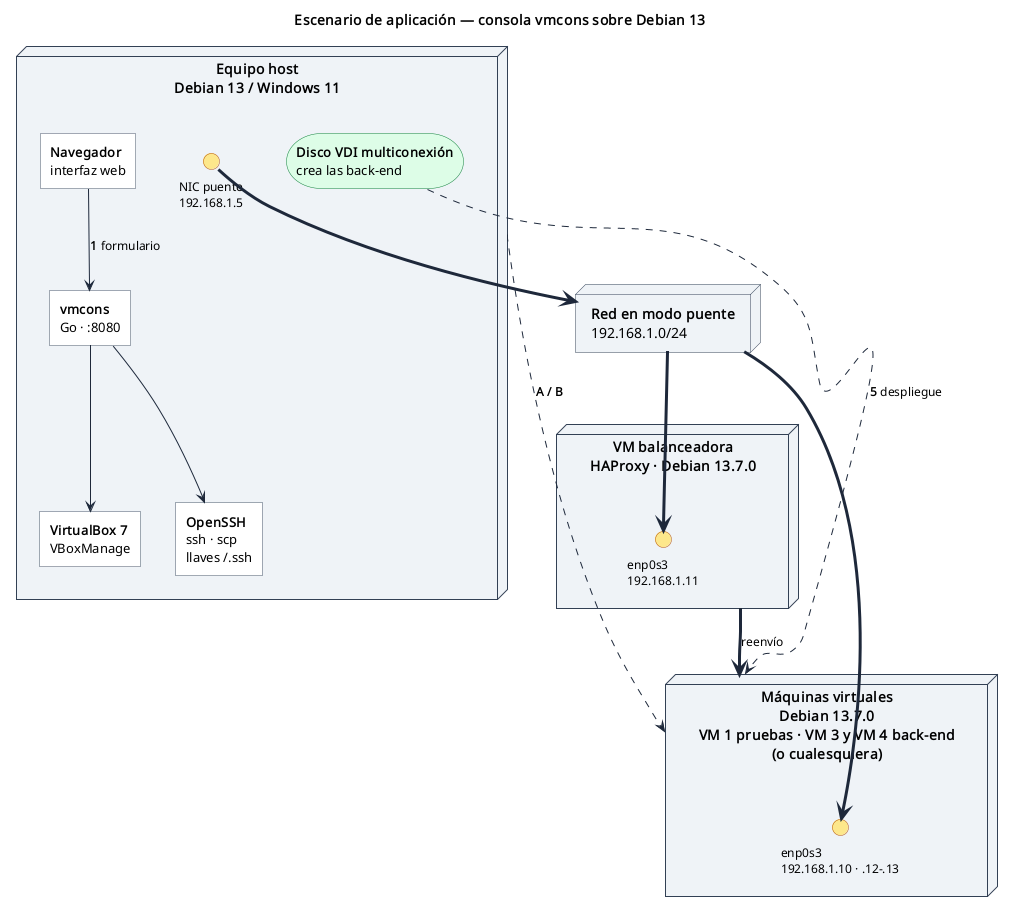
\includegraphics[width=\textwidth]{images/escenario}
  \caption{Escenario utilizado para desarrollar y probar la solución:
  equipo host, software de virtualización, máquinas virtuales con su
  sistema operativo, interfaces de red y direcciones IP, mecanismos de
  comunicación, disco de almacenamiento y flujo general de la
  automatización. El enlace A/B es el mecanismo de comunicación con la
  VM: A corresponde a las Guest Additions (solo antes de instalar SSH)
  y B al acceso por SSH con llaves (después, de forma exclusiva).}
  \label{fig:escenario}
\end{figure*}

% Flujo de proceso: se declara junto a la Figura 1 para que la
% colocación de la figura sea anterior al final de la sección.
% Fuente: docs/diagramas/flujo-procesos.puml (regenerar con «task diagramas»).
\begin{figure*}[!t]
  \centering
  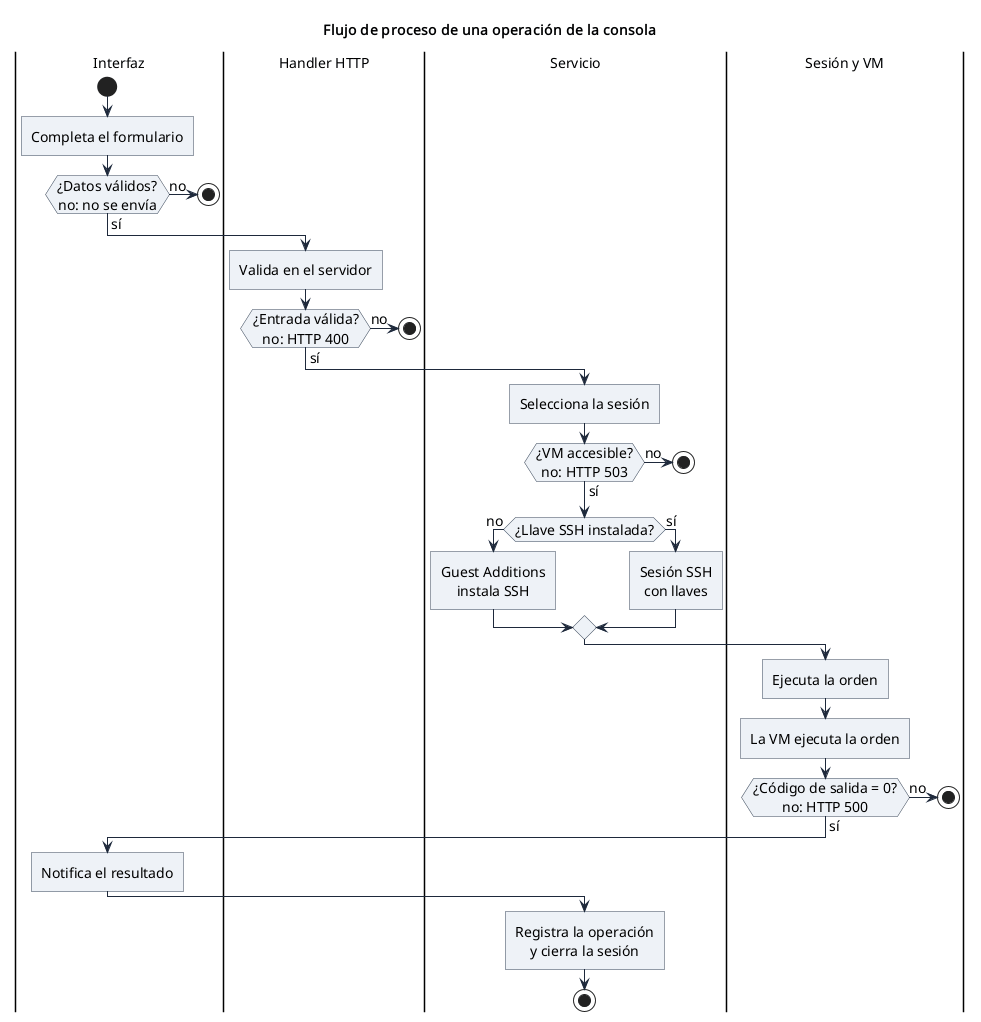
\includegraphics[width=0.95\textwidth]{images/flujo-procesos}
  \caption{Flujo de proceso de una operación solicitada desde la interfaz,
  con los responsables de cada etapa: interfaz, validación en el servidor,
  selección de sesión, ejecución no interactiva y notificación del
  resultado o del error técnico.}
  \label{fig:flujo-proceso}
\end{figure*}

\subsubsection{Descripción del Escenario}
\label{sec:desc-escenario}

La solución se desarrolla y se prueba sobre el escenario de la
\cref{fig:escenario}. El \emph{equipo host} es el equipo físico donde se
instala Oracle VM VirtualBox~7 y se ejecuta la consola \texttt{vmcons};
su sistema operativo puede ser GNU/Linux Debian~13 o Windows~11, ya que
la consola se compila como un binario único sin dependencias en tiempo de
ejecución. La consola publica la interfaz web en el puerto \texttt{8080}
y es accedida desde un navegador instalado en el mismo equipo.

La red física funciona en modo puente (bridge) sobre la subred
\texttt{192.168.1.0/24}, con un servidor DHCP/DNS en \texttt{192.168.1.1}.
La tarjeta de red del anfitrión recibe \texttt{192.168.1.5} y las
máquinas virtuales reciben direcciones de la misma subred en su
interfaz \texttt{enp0s3}: \texttt{192.168.1.10} a \texttt{192.168.1.13}.
Al estar en modo puente, las VM quedan visibles en la red local con una
dirección propia, lo que permite probar servicios de red reales como SSH
o HAProxy sin reglas de reenvío de puertos.

Todas las máquinas virtuales ejecutan GNU/Linux Debian~13.7.0. El
balanceador ocupa un nodo propio en la \cref{fig:escenario} porque es la
máquina del módulo de HAProxy: recibe las peticiones en
\texttt{192.168.1.11} y las reenvía, a través de la misma red, a los
servidores del back-end. Las restantes se resumen en un único contenedor
etiquetado como «o cualesquiera»: la VM~1 es la máquina de pruebas sobre
la que se ejecutan los módulos de preparación del sistema, gestión de
usuarios y servicios con systemd, y la VM~3 y la VM~4 son los servidores
del back-end; la consola abre sesión con la máquina que corresponda en
cada operación, de modo que el conjunto de VM cambia según las pruebas.
Estas últimas se crean a partir de un \emph{disco virtual VDI
de multiconexión} (multiattach) con carga diferencial guardado en el
anfitrión, de modo que cada back-end arranca desde la misma imagen base
sin duplicar el disco y puede añadirse o eliminarse una máquina más
utilizando el mismo archivo.

\subsubsection{Mecanismo de Comunicación}
\label{sec:mecanismo-com}

La consola se comunica con la máquina virtual mediante dos mecanismos,
marcados como \textbf{A} y \textbf{B} en la \cref{fig:escenario}.

El \textbf{mecanismo A} se basa en las Guest Additions
\parencite{guestadditions} y se usa \emph{únicamente antes} de instalar
SSH. La consola obtiene la dirección IP de la VM con
\texttt{VBoxManage guestproperty get} sobre la propiedad
\texttt{/VirtualBox/GuestInfo/Net/0/V4/IP}, genera el par de llaves en el
anfitrión, instala \texttt{openssh-server}, copia la llave pública al
archivo \texttt{authorized\_keys} del usuario \texttt{root} y deshabilita
el acceso por contraseña. Las órdenes se ejecutan con
\texttt{VBoxManage guestcontrol run} y los archivos se transfieren con
\texttt{guestcontrol copyto}.

El \textbf{mecanismo B} es el acceso por SSH con llaves de autenticación
\parencite{rfc4252}, mediante el cliente OpenSSH del anfitrión
(\texttt{ssh} y \texttt{scp}). Una vez instalado SSH, \emph{toda} la
comunicación posterior entre la consola y la máquina se realiza por este
canal, tal como exige el enunciado: el mecanismo A deja de utilizarse y
la consola trabaja de forma exclusiva sobre SSH, con la llave privada
resguardada en el equipo anfitrión.

\subsubsection{Flujo General de la Automatización}
\label{sec:flujo-escenario}

Todo módulo de la consola recorre el mismo flujo: (1) el usuario completa
el formulario en el navegador y lo envía; (2) la consola valida los datos
y selecciona la sesión adecuada, es decir, decide si aún necesita Guest
Additions o si ya puede trabajar por SSH; (3) ejecuta la orden de forma
no interactiva sobre la máquina virtual; (4) la máquina devuelve la
salida y la consola notifica el resultado, o bien presenta un mensaje de
error comprensible junto con la información técnica de diagnóstico; y (5)
el disco multiconexión permite ampliar el escenario creando nuevas
back-end para las pruebas de balanceo de carga.

% ------------------------------------------------------------
% 3.2 Arquitectura de la solución
% ------------------------------------------------------------
\subsection{Arquitectura de la Solución}
\label{sec:arquitectura}

\subsubsection{Visión General de la Aplicación}
\label{sec:vision-general}

La consola es una aplicación web escrita en Go que se sirve con el
paquete estándar \texttt{net/http}. La interfaz está organizada por
módulos ---preparación del sistema, gestión de usuarios, servicios con
systemd y balanceo de carga---, y cada módulo presenta un formulario con
los campos y las casillas de verificación que la operación requiere.

Toda operación sigue el ciclo de la \cref{fig:flujo-proceso}: validación
en el cliente para dar respuesta inmediata, validación en el servidor
sobre los parámetros crudos (que es la que realmente decide), selección
de la sesión, ejecución no interactiva de la orden y notificación del
resultado. Si la validación falla, la operación \emph{no} llega a la
máquina virtual y la respuesta indica el campo y el motivo; si la orden
se ejecuta y termina con un código de salida distinto de cero, la
respuesta conserva la orden ejecutada, el código de salida y la salida de
error estándar para que el usuario pueda diagnosticar el problema. Las
respuestas son documentos JSON con un campo \texttt{ok}, un
\texttt{mensaje} comprensible y, cuando falla, los campos
\texttt{operacion} y \texttt{tecnico} con el detalle técnico.

\subsubsection{Estructura del Proyecto}
\label{sec:estructura-proyecto}

El proyecto se organiza en capas para que el núcleo de la aplicación no
dependa de VirtualBox, de las Guest Additions ni de OpenSSH:

\begin{itemize}
  \item \texttt{main.go}: único punto de composición. Aquí se
  instancian los adaptadores y se inyectan a los servicios y a los
  manejadores HTTP.
  \item \texttt{internal/core/domain}: tipos del dominio
  (\texttt{Command}, \texttt{Result}, \texttt{Target},
  \texttt{MachineState} y \texttt{ExitError}) sin dependencias externas.
  \item \texttt{internal/core/ports}: interfaces \texttt{Executor},
  \texttt{Machine}, \texttt{Connector} y \texttt{Session} que expresan lo
  que la aplicación necesita del exterior.
  \item \texttt{internal/adapters}: las implementaciones concretas
  \texttt{localproc} (procesos del sistema operativo anfitrión),
  \texttt{vbox} (VirtualBox y Guest Additions) y \texttt{ssh} (cliente
  OpenSSH).
  \item \texttt{internal/services}: los casos de uso de cada módulo;
  dependen solo de los puertos del núcleo.
  \item \texttt{internal/handlers}: enrutan las peticiones HTTP y
  validan las entradas; no contienen lógica de negocio.
  \item \texttt{web}: los módulos HTML y los archivos estáticos de la
  interfaz.
\end{itemize}

Los adaptadores traducen su vocabulario al dominio: por ejemplo,
\texttt{vbox} convierte el estado \texttt{poweroff} de VirtualBox en
\texttt{domain.MachinePoweredOff}, de modo que el núcleo nunca necesita
saber qué tecnología se está utilizando. La regla de dependencia es
simple: el núcleo no importa adaptadores, los adaptadores importan el
núcleo y la composición ocurre únicamente en \texttt{main.go}.

\subsubsection{Decisiones Tomadas Durante el Desarrollo}
\label{sec:decisiones}

Las decisiones principales del diseño son las siguientes.

\emph{Binarios del sistema, no librerías nativas.} El SDK de VirtualBox
exige COM en Windows y bindings específicos en GNU/Linux; en su lugar se
invoca \texttt{VBoxManage}, oficial y multiplataforma, y para SSH se usa
el cliente incluido en el sistema en lugar de una implementación en Go
\parencite{donovan}.

\emph{Errores tipados.} Las órdenes que terminan con un código distinto
de cero producen un \texttt{domain.ExitError} que conserva el código, la
salida estándar y la salida de error; el núcleo lo entiende sin importar
qué adaptador lo originó.

\emph{Validación antes de ejecutar y en el servidor.} Las direcciones se
modelan con \texttt{net/netip.Addr}, los nombres de usuario y de host se
comprueban con expresiones regulares y ninguna entrada cruda llega a la
máquina virtual.

\emph{Un solo flujo para los siete módulos.} Todos comparten el ciclo
entrada, validación, sesión, ejecución, clasificación y notificación, lo
que uniformiza los mensajes de error y hace que las pruebas sean
repetibles.

\emph{Calidad de código verificable.} El flujo de trabajo exige
formateo con \texttt{gofumpt}, análisis con \texttt{golangci-lint} y
pruebas con detector de condiciones de carrera antes de cada commit.

\FloatBarrier

% ============================================================
% 4. IMPLEMENTACIÓN
% (preparación del sistema, gestión de usuarios, gestión de
%  demonios con systemd y balanceo de carga con HAProxy)
% ============================================================
\section{Implementación}
\label{sec:implementacion}

La capa HTTP está implementada: los catorce recursos de la
\cref{tab:api-rest} tienen su manejador, la validación del servidor
aplica las reglas descritas en la \cref{sec:contrato-rest} y cada
petición se responde con el modelo JSON de la
\cref{sec:vision-general}. El descubrimiento de sesión
expone \texttt{GET /api/session} y el módulo de paquetes ya ejecuta APT
sobre la máquina. Los demás casos de uso, mientras no se conecten,
responden \texttt{501} con un mensaje comprensible, de modo que la
interfaz puede integrarse sin esperar a la ejecución real. Las pruebas
cubren el 96.0\,\% de los manejadores y el 100\,\% de los servicios.

% ------------------------------------------------------------
% 4.1 Preparación del sistema
% ------------------------------------------------------------
\subsection{Preparación del Sistema}
\label{sec:preparacion}

\subsubsection{Instalación y Eliminación de Aplicaciones}
\label{sec:apt}

El módulo de paquetes se apoya en el recurso \texttt{/api/packages}. El
formulario indica la acción y el nombre del paquete; el servidor valida
el nombre con la regla de paquetes APT antes de tocar la máquina. La
instalación ejecuta \texttt{apt-get install -y} y la eliminación
\texttt{apt-get remove -y} sobre ese nombre, con
\texttt{DEBIAN\_FRONTEND=noninteractive} para que APT no solicite
confirmaciones aunque la sesión no sea interactiva.

Cada operación abre una sesión con el conector disponible, la cierra al
terminar y clasifica el resultado. Si el código de salida es cero,
responde \texttt{201} al instalar (con \texttt{Location}) o
\texttt{204} al eliminar, e incluye la salida relevante; si es distinto
de cero, responde \texttt{500} conservando la orden ejecutada, el
código de salida y el \texttt{stderr} para el diagnóstico. El listado
usa \texttt{dpkg-query} y filtra por el estado
\texttt{install ok installed}. La cobertura del servicio de paquetes es
del 100\,\%.

\subsubsection{Configuración de la Llave de Acceso SSH para el Usuario Root}
\label{sec:ssh-root}
% TODO: creación de llaves para root, instalación de la llave pública en
% authorized_keys, deshabilitación del acceso por login y password,
% descarga de la llave privada y mensaje de recomendación de uso
% correcto de la llave.

\subsubsection{Personalización de la Entrada del Sistema}
\label{sec:issue}
% TODO: configuración de /etc/issue con opciones para nombre del host,
% fecha, hora, dirección IP y mensaje personalizado de inicio de sesión.

\subsubsection{Asignación del Nombre de Host y Actualización del Archivo de Hosts}
\label{sec:hostname}
% TODO: establecimiento del nombre de host y actualización del
% contenido de /etc/hosts.

% ------------------------------------------------------------
% 4.2 Gestión de usuarios
% ------------------------------------------------------------
\subsection{Gestión de Usuarios}
\label{sec:usuarios}

\subsubsection{Creación de Usuarios y Privilegios de sudo}
\label{sec:crear-usuario}
% TODO: creación de usuario con casilla de verificación para privilegios
% sudo; casilla para generar el par de llaves criptográficas, instalar
% la llave pública y habilitar el descargue de la llave privada;
% deshabilitación del acceso por login y password al habilitar SSH.

\subsubsection{Eliminación de Usuarios}
\label{sec:eliminar-usuario}
% TODO: eliminación de usuarios con casilla de verificación que indica
% si también deben eliminarse todos sus archivos.

% ------------------------------------------------------------
% 4.3 Gestión de demonios con systemd
% ------------------------------------------------------------
\subsection{Gestión de Demonios con systemd}
\label{sec:systemd}
% TODO: configuración de una aplicación como servicio de systemd
% (por ejemplo, la aplicación web del catálogo de libros): transferencia
% de los archivos requeridos a la máquina virtual y gestión de
% permisos; botones start, stop, restart, status, enable y disable;
% prueba complementaria con el script que agrega fecha y hora a un
% archivo.

% ------------------------------------------------------------
% 4.4 Balanceo de carga con HAProxy
% ------------------------------------------------------------
\subsection{Gestión de un Balanceador de Carga con HAProxy}
\label{sec:haproxy}
% TODO: mecanismo para agregar y eliminar un servidor del back-end del
% balanceador de carga; verificación del balanceo con back-end creadas
% manualmente con VirtualBox (entorno de pruebas, fuera de la consola).

% ============================================================
% 5. PRUEBAS
% ============================================================
\section{Pruebas}
\label{sec:pruebas}

\subsection{Diseño de las Pruebas}
\label{sec:diseno-pruebas}

Cada capacidad de la solución se verifica con una prueba que sigue la
misma estructura: se comprueba y se registra el \emph{estado anterior}
de la máquina con órdenes ejecutadas fuera de la consola ---terminal de
la VM, de otra VM o del anfitrión---, se realiza la operación desde la
interfaz web y se vuelve a comprobar el \emph{estado posterior} con las
mismas órdenes. La comprobación externa es deliberada: si el estado
posterior se leyera solo en la interfaz, una respuesta incorrecta del
servidor podría pasar por un éxito. Cada prueba se graba en video desde
el navegador y la terminal al mismo tiempo, de modo que el estado
anterior y el posterior quedan visibles en el mismo registro.

El entorno es el de la \cref{fig:escenario}: el anfitrión con
VirtualBox~7.2 y la consola; el servidor S1 (\texttt{192.168.1.29}),
preparado desde el disco de multiconexión con Debian~13.7.0 en modo
puente y el servicio de imágenes en el puerto~8000, que se usa además
para las pruebas de preparación del sistema; el servidor S2
(\texttt{192.168.1.30}), con la misma distribución y el mismo servicio,
que completa el back-end y sirve para el cambio de máquina; y el
balanceador B (\texttt{192.168.1.32}), con HAProxy sobre Debian~13.7.0.
En el anfitrión se usa \texttt{oha}~1.16 para generar carga sobre el
balanceador. Las direcciones IP se obtienen por DHCP y no se fijan en la
prueba: la consola las descubre en tiempo de ejecución.

Las \cref{tab:diseno-pruebas,tab:diseno-pruebas-b}
resumen las veintidós pruebas diseñadas. Las pruebas P05 y P16 incluyen, además
del camino correcto, el camino de error: un paquete que no existe en los
repositorios y la baja repetida de un servidor del back-end; P22 añade la
carga concurrente con \texttt{oha} para observar el reparto entre los dos
servidores.

\begin{table*}[!tp]
  \centering
  \caption{Diseño de las pruebas (parte 1 de 2): estado anterior,
  operación y estado posterior esperado de cada elemento de la solución.}
  \label{tab:diseno-pruebas}
  \scriptsize
  \begin{tabularx}{\textwidth}{@{}l >{\raggedright\arraybackslash}p{2.3cm}
      >{\raggedright\arraybackslash}X >{\raggedright\arraybackslash}X
      >{\raggedright\arraybackslash}X
      >{\raggedright\arraybackslash}p{1.0cm}@{}}
    \hline
    ID & Capacidad & Estado anterior & Operación desde la consola &
    Estado posterior esperado & Video \\
    \hline
    P01 & Registro de la máquina & S2 apagada y sin registrar; sin
    llave de root en el anfitrión. & Encender desde el selector y
    registrar con el usuario y la contraseña de la VM. &
    \texttt{/api/session} informa la IP y el conector \texttt{ssh}; la
    máquina aparece registrada y no vuelve a pedir credenciales. & V01 \\
    P02 & Diagnóstico del registro & VM con Guest Additions~6.0 sobre
    VirtualBox~7.2, cuyo \texttt{guestcontrol} rechaza la contraseña. &
    Enviar las credenciales en el modal y abrir el diagnóstico. &
    Mensaje comprensible y diagnóstico con versión de Guest Additions,
    puerto 22 y usuario con sesión; el registro se completa por SSH con
    \texttt{sshpass}. & V02 \\
    P03 & Instalar paquete & \texttt{dpkg-query -W htop} responde que no
    está instalado. & Formulario de paquetes: instalar \texttt{htop}. &
    \texttt{htop} figura como \texttt{install ok installed}, aparece en
    el listado y la ficha muestra el código de salida cero. & V03 \\
    P04 & Eliminar paquete & \texttt{htop} instalado. & Eliminar
    \texttt{htop} y confirmar en el aviso. & \texttt{htop} ya no está
    instalado, desaparece del listado y la ficha describe la orden
    ejecutada. & V04 \\
    P05 & Error de APT & Paquete \texttt{paquete-inexistente} no
    disponible en los repositorios. & Intentar instalarlo. & Respuesta
    \texttt{500} con mensaje comprensible, código de salida de APT y
    \texttt{stderr} en el detalle técnico; la máquina queda sin cambios.
    & V05 \\
    P06 & Llave de \texttt{root} & Sin
    \texttt{/etc/ssh/\allowbreak sshd\_config.d/\allowbreak
    99-vmcons.conf} ni llave en el
    anfitrión. & Generar la llave y descargar la privada. &
    \texttt{authorized\_keys} con permisos \texttt{700}/\texttt{600};
    \texttt{sshd -T} informa \texttt{passwordauthentication no} y
    \texttt{permitrootlogin prohibit-password}; la descarga entrega un
    archivo adjunto y la interfaz recomienda resguardarlo. & V06 \\
    P07 & Acceso por contraseña & Contraseña de \texttt{root}
    deshabilitada por P06. & \texttt{ssh -o \allowbreak
    PubkeyAuthentication=no \allowbreak root@IP}. & El intento por
    contraseña se rechaza y el acceso con \texttt{-i llave} funciona.
    & V07 \\
    P08 & \texttt{/etc/issue} & Banner original de Debian, que la
    consola muestra como texto ajeno con las casillas desactivadas. &
    Escribir un mensaje y marcar nombre de host, fecha, hora e IP. &
    \texttt{cat /etc/issue} muestra las etiquetas y las secuencias de
    \texttt{agetty}; la consola de inicio de sesión las expande. & V08 \\
    P09 & Nombre de host y \texttt{/etc/hosts} & \texttt{hostname}
    devuelve \texttt{debian} y \texttt{/etc/hosts} no menciona la IP de
    la VM. & Asignar \texttt{vmcons-lab} con la casilla de actualizar
    \texttt{/etc/hosts}. & \texttt{hostname} devuelve
    \texttt{vmcons-lab}, \texttt{/etc/hosts} conserva
    \texttt{localhost} y agrega «IP nombre»; el cambio persiste tras
    reiniciar. & V09 \\
    P10 & Crear usuario con \texttt{sudo} y llaves & \texttt{id alumno}
    responde que no existe la cuenta. & Crear \texttt{alumno} con las
    casillas de \texttt{sudo} y de llaves, y descargar la privada. &
    UID entre 1000 y 65533, grupo \texttt{sudo},
    \texttt{authorized\_keys} del usuario con \texttt{700}/\texttt{600}
    y contraseña bloqueada; la cuenta aparece en el listado. & V10 \\
    P11 & Eliminar usuario & \texttt{alumno} existe y tiene
    \texttt{/home/alumno}. & Eliminar con la casilla de borrar archivos.
    & \texttt{id alumno} falla, \texttt{/home/alumno} ya no existe y la
    llave del anfitrión se elimina; la cuenta sale del listado. & V11 \\
    \hline
  \end{tabularx}
\end{table*}

\begin{table*}[!tp]
  \centering
  \caption{Diseño de las pruebas (parte 2 de 2): estado anterior,
  operación y estado posterior esperado de cada elemento de la solución.}
  \label{tab:diseno-pruebas-b}
  \scriptsize
  \begin{tabularx}{\textwidth}{@{}l >{\raggedright\arraybackslash}p{2.3cm}
      >{\raggedright\arraybackslash}X >{\raggedright\arraybackslash}X
      >{\raggedright\arraybackslash}X
      >{\raggedright\arraybackslash}p{1.0cm}@{}}
    \hline
    ID & Capacidad & Estado anterior & Operación desde la consola &
    Estado posterior esperado & Video \\
    \hline
    P12 & Desplegar una unidad & La aplicación del catálogo no está en
    la VM ni tiene unidad. & Subir el ejecutable y el archivo
    \texttt{.service} con modo \texttt{0755} y propietario. &
    \texttt{systemctl cat} muestra la unidad, \texttt{daemon-reload}
    queda aplicado y el listado la informa inactiva y deshabilitada.
    & V12 \\
    P13 & Ciclo de vida de la unidad & Unidad inactiva y deshabilitada.
    & \texttt{start}, \texttt{enable}, \texttt{restart},
    \texttt{stop} y \texttt{disable} desde los botones. &
    \texttt{systemctl is-active} y \texttt{is-enabled} reflejan cada
    paso; \texttt{status} muestra un PID distinto tras el reinicio.
    & V13 \\
    P14 & Script de la precondición e) & Unidad del script inactiva y
    archivo de registro sin líneas del día. & Iniciar y reiniciar la
    unidad. & Cada ejecución agrega una línea con la fecha y la hora;
    tras el reinicio hay dos líneas nuevas y un PID distinto. & V14 \\
    P15 & Agregar servidores al back-end & \texttt{backend}
    \texttt{vmcons\_app} vacío en el balanceador. & Agregar
    \texttt{192.168.1.29:8000} y \texttt{192.168.1.30:8000}. & Dos
    líneas \texttt{server srv\_\dots\ check}, configuración válida con
    \texttt{haproxy -c}, servicio recargado y \texttt{curl} al
    balanceador atendido por los dos servidores. & V15 \\
    P16 & Eliminar servidores del back-end & S1 y S2 en el back-end
    del balanceador. & Eliminar S1 y después S2. & La línea de S1
    desaparece y el tráfico solo llega a S2; sin servidores el
    balanceador responde \texttt{503} y repetir la baja da
    \texttt{404}. & V16 \\
    P17 & Historial y persistencia & Base con operaciones anteriores de
    la sesión de pruebas. & Ejecutar tres operaciones y consultar la
    pestaña Historial con filtros de texto, fecha, máquina y módulo;
    exportar a CSV. & Las tres operaciones aparecen con descripción
    legible; los filtros acotan el resultado; el CSV coincide y las
    filas sobreviven al reinicio de la consola. & V17 \\
    P18 & Cambio de máquina vinculada & S1 vinculada y listados
    cargados en varias pestañas. & Vincular S2 desde el selector.
    & La barra muestra la IP de S2 y los listados se recargan sin
    conservar filas de S1. & V18 \\
    P19 & Estado de HAProxy & HAProxy con la configuración por omisión,
    sin bloques \texttt{backend}. & Abrir el módulo HAProxy y consultar
    el estado. & La tarjeta indica que requiere configuración con el
    problema «no tiene bloques backend»; el estado informa el binario,
    la configuración válida, el servicio y el puerto. & V19 \\
    P20 & Configuración rápida & HAProxy sin \texttt{frontend} ni
    \texttt{backend} propios. & Pulsar \textbf{Configuración rápida}.
    & \texttt{haproxy.cfg} con \texttt{frontend vmcons\_front} en el
    puerto~80 y \texttt{backend vmcons\_app}; copia
    \texttt{.bak-\dots}, \texttt{haproxy -c} válida, servicio activo y
    tarjeta con la URL de entrada. & V20 \\
    P21 & Métricas de los servidores & S1 y S2 agregados al back-end.
    & Abrir el detalle de cada servidor y recargar. & Estado
    \texttt{UP}, peso, activo, sesiones, cola, bytes enviados y
    recibidos, \texttt{L4OK}, duración del chequeo y tiempos; los
    totales crecen con el tráfico. & V21 \\
    P22 & Balanceo bajo carga y URL de entrada & Totales similares en S1
    y S2. & Copiar la URL del balanceador y ejecutar
    \texttt{oha --no-tui -n 600 -c 30 http://192.168.1.32/}. & Todas las
    respuestas son \texttt{2xx}; ambos servidores suman unas 300
    peticiones y el máximo de sesiones sube; la URL copiada abre la
    aplicación. & V22 \\
    \hline
  \end{tabularx}
\end{table*}

\subsection{Resultados y Evidencias}
\label{sec:resultados-pruebas}

\subsubsection{Verificación Automática}
\label{sec:resultados-automaticos}

Las pruebas automatizadas verifican la lógica que no depende de una
máquina real: la validación de entradas, la traducción de errores, el
descubrimiento y la selección del conector, la construcción de las
órdenes, el manejo de los recursos HTTP, la persistencia, la caché y el
historial. La \cref{tab:cobertura} resume el resultado; las órdenes se
ejecutan con las tareas del proyecto (\texttt{task test},
\texttt{task lint}, \texttt{task openapi} y \texttt{pnpm test}).

\begin{table}[!t]
  \centering
  \caption{Resultado de las pruebas automatizadas.}
  \label{tab:cobertura}
  \footnotesize
  \begin{tabularx}{\columnwidth}{@{}l >{\raggedleft\arraybackslash}X@{}}
    \hline
    Paquete & Cobertura de sentencias \\
    \hline
    \texttt{core/domain} & 100.0\,\% \\
    \texttt{adapters/localproc} & 100.0\,\% \\
    \texttt{httpcache} & 100.0\,\% \\
    \texttt{handlers} & 98.5\,\% \\
    \texttt{services} & 94.9\,\% \\
    \texttt{adapters/ssh} & 100.0\,\% \\
    \texttt{adapters/vbox} & 100.0\,\% \\
    Ejecutable (\texttt{main}) & 82.5\,\% \\
    \hline
  \end{tabularx}
\end{table}

Las pruebas automatizadas terminan sin fallos y el análisis estático no
reporta incidencias. Los paquetes internos alcanzan el 100\,\% salvo
\texttt{handlers} (98.5\,\%) y \texttt{services} (94.9\,\%), donde las
sentencias restantes son ramas de error de restauración, cifrado y cierre
de sesión que exigen fallos encadenados. Los adaptadores
y los servicios se prueban con ejecutores y sesiones falsos que devuelven
salidas realistas de \texttt{VBoxManage} y \texttt{ssh}, y los
manejadores con peticiones HTTP simuladas; las pruebas de campo P01 a P22
completan lo que solo tiene sentido frente a un hipervisor real. El
paquete del ejecutable queda en el 82.5\,\%: su función de arranque y el
servidor que queda escuchando no se pueden ejercitar en una prueba
unitaria sin abrir un puerto. El contrato OpenAPI se valida sin errores y
ninguna de sus rutas devuelve \texttt{501}.

\subsubsection{Pruebas de Campo}
\label{sec:resultados-campo}

Las veintidós pruebas de las \cref{tab:diseno-pruebas,tab:diseno-pruebas-b} se ejecutan sobre
el escenario y se graban en video, con el nombre \texttt{V01} a
\texttt{V22} según la tabla. Cada grabación empieza con la comprobación
del estado anterior en la terminal, continúa con la operación en la
interfaz ---el formulario, la validación y la ficha del panel de
resultado--- y termina con la comprobación del estado posterior en la
misma terminal, de modo que la evidencia cubre el ciclo completo y no
solo la respuesta de la consola.

La ejecución del 26 de octubre de 2026 cubrió las veintidós pruebas
sobre los servidores S1 (\texttt{192.168.1.29}) y S2
(\texttt{192.168.1.30}) y el balanceador B (\texttt{192.168.1.32}). Las
máquinas se renombraron a S1, S2 y B para la grabación y el DHCP les
asignó esas direcciones; el registro de la ejecución conserva los nombres
y las direcciones anteriores. Las pruebas P01 a P18 se ejecutaron con el
arnés automatizado, que comprobó
el estado anterior por SSH, ejecutó la operación y verificó el estado
posterior con la misma conexión; P19 a P22 se verificaron en la misma
sesión desde la interfaz y el socket de estadísticas, con \texttt{oha}
como generador de carga. Las veintidós terminaron conformes; la
\cref{tab:resultados-campo} resume lo observado
y el detalle completo, con las salidas y los códigos de cada llamada,
está en \texttt{docs/resultados-pruebas.md}. Las pruebas restauran el
estado que modifican: la llave privada del anfitrión, el nombre de host,
\texttt{/etc/issue}, la unidad temporal y los servidores del
balanceador quedaron como estaban antes de la ejecución, y la
configuración de HAProxy se recuperó de la copia guardada antes de P19.

\begin{table*}[!t]
  \centering
  \caption{Resultados observados en las pruebas de campo.}
  \label{tab:resultados-campo}
  \scriptsize
  \begin{tabularx}{\textwidth}{@{}l >{\hsize=0.8\hsize}X >{\hsize=0.9\hsize}X >{\hsize=1.3\hsize}X c@{}}
    \hline
    Prueba & Antes & Operación & Después & Resultado \\
    \hline
    P01 & S2 sin registrar & \texttt{POST /api/session/register} & \texttt{registrada=true}; Guest Additions 6.0.0 & Conforme \\
    P02 & S2 registrada & \texttt{GET /api/session/diagnostico} & Red puente, IP \texttt{.30}, SSH abierto y aviso de Guest Additions & Conforme \\
    P03 & \texttt{tree} no instalado & \texttt{POST /api/packages} & \texttt{install ok installed} & Conforme \\
    P04 & \texttt{tree} instalado & \texttt{DELETE /api/packages/tree} & \texttt{dpkg-query}: no encontrado & Conforme \\
    P05 & \texttt{tree} eliminado & Alta de paquete inexistente & \texttt{500} con código 1 y \texttt{stderr} de APT & Conforme \\
    P06 & Sin llave privada en el anfitrión & \texttt{POST} y \texttt{GET /api/keys/root} & SSH con la llave nueva; \texttt{passwordauthentication no} & Conforme \\
    P07 & Contraseña deshabilitada & SSH sin autenticación por llave & \texttt{Permission denied (publickey)} & Conforme \\
    P08 & \texttt{/etc/issue} original & \texttt{PUT /api/issue} & Mensaje con escapes \texttt{\textbackslash n}, \texttt{\textbackslash d}, \texttt{\textbackslash t} y \texttt{\textbackslash 4} & Conforme \\
    P09 & Nombre de host \texttt{base} & \texttt{PUT /api/hostname} & \texttt{vmcons-lab} y entrada en \texttt{/etc/hosts} & Conforme \\
    P10 & Usuario \texttt{alumno} inexistente & \texttt{POST /api/users} & UID 1001, grupo \texttt{sudo}, llave 0600 y descarga & Conforme \\
    P11 & \texttt{alumno} con directorio & \texttt{DELETE /api/\allowbreak users/\allowbreak alumno?files=true} & Usuario y \texttt{/home/alumno} eliminados & Conforme \\
    P12 & Unidad inexistente & \texttt{PUT /api/units/vmcons-demo.service} & Unidad creada; \texttt{daemon-reload} & Conforme \\
    P13 & Unidad inactiva & Activar, habilitar, reiniciar y detener & \texttt{active}, \texttt{enabled}, \texttt{202}, \texttt{inactive} & Conforme \\
    P14 & Sin ejecuciones del script & Iniciar y reiniciar la unidad & Cinco líneas con fecha y hora ISO-8601 & Conforme \\
    P15 & Back-end sin servidores & \texttt{POST /api/\allowbreak haproxy/\allowbreak backend/\allowbreak servers} con S1 y S2 & Líneas \texttt{srv\_192\_168\_1\_29\_8000} y \texttt{srv\_192\_168\_1\_30\_8000}; \texttt{haproxy -c} válida y \texttt{curl} 200 & Conforme \\
    P16 & S1 y S2 en el back-end & \texttt{DELETE /api/\allowbreak haproxy/\allowbreak backend/\allowbreak servers} & S1 fuera y solo S2 atiende; sin servidores \texttt{503} y repetir 404 & Conforme \\
    P17 & Operaciones anteriores & \texttt{GET /api/historial?q=paquetes} & Operaciones con descripción legible & Conforme \\
    P18 & S1 vinculada & \texttt{PUT /api/session} con S2 & IP \texttt{.29} sustituida por \texttt{.30} & Conforme \\
    P19 & Configuración sin \texttt{backend} & \texttt{GET /api/haproxy/status} & Problema «no tiene bloques backend»; binario, configuración, servicio y puerto informados & Conforme \\
    P20 & Sin \texttt{frontend} ni \texttt{backend} & \texttt{POST /api/haproxy/configurar} & \texttt{vmcons\_front} en el puerto 80, \texttt{vmcons\_app}, copia \texttt{.bak-\dots} y servicio activo & Conforme \\
    P21 & S1 y S2 agregados & \texttt{GET /api/\allowbreak haproxy/\allowbreak backend/\allowbreak servers} & \texttt{UP}, peso 1, \texttt{L4OK}, sesiones, bytes y más de 13\,000 peticiones acumuladas & Conforme \\
    P22 & Totales similares & \texttt{oha --no-tui -n 600 -c 30} & 100\,\% de respuestas \texttt{2xx}; unos 300 registros más en cada servidor & Conforme \\
    \hline
  \end{tabularx}
\end{table*}

Los videos se entregan junto con el trabajo, fuera de este documento,
con el nombre que indica la tabla. Las capturas de la interfaz que
acompañan al informe están en la Sección~IV, donde se explica el módulo
correspondiente.

\begin{table}[!t]
  \centering
  \caption{Videos de las pruebas de campo, entregados por separado.}
  \label{tab:evidencias}
  \footnotesize
  \begin{tabularx}{\columnwidth}{@{}l X@{}}
    \hline
    Video & Contenido \\
    \hline
    V01--V02 & Registro y diagnóstico de la máquina \\
    V03--V05 & Paquetes: instalar, eliminar y error de APT \\
    V06--V07 & Llave de \texttt{root} y bloqueo de la contraseña \\
    V08--V09 & \texttt{/etc/issue} y nombre de host \\
    V10--V11 & Creación y eliminación de usuarios \\
    V12--V14 & Despliegue y ciclo de vida con systemd \\
    V15--V16 & Back-end de HAProxy: alta y baja \\
    V17--V18 & Historial y cambio de máquina \\
    V19--V22 & HAProxy: estado, configuración rápida, métricas y carga \\
    \hline
  \end{tabularx}
\end{table}

% Las tablas de esta sección no deben aparecer dentro de las conclusiones.
\FloatBarrier

% ============================================================
% 6. CONCLUSIONES
% (problemas encontrados, herramientas de IA empleadas y
%  conclusiones del trabajo)
% ============================================================
\section{Conclusiones}
\label{sec:conclusiones-apartado}

% ------------------------------------------------------------
% 6.1 Problemas encontrados y soluciones
% ------------------------------------------------------------
\subsection{Problemas Encontrados y Soluciones}
\label{sec:problemas}
% TODO: describir los principales problemas surgidos durante el
% desarrollo (por ejemplo: comunicación inicial con la VM, permisos de
% sudo, configuración de HAProxy, manejo de errores de comandos, etc.)
% y la forma en que fueron solucionados.

% ------------------------------------------------------------
% 6.2 Herramientas de inteligencia artificial utilizadas
% ------------------------------------------------------------
\subsection{Herramientas de Inteligencia Artificial Utilizadas}
\label{sec:herramientas-ia}
% TODO: listar las herramientas de IA empleadas (por ejemplo, agentes
% de código) y detallar para qué fueron utilizadas.

% ------------------------------------------------------------
% 6.3 Conclusiones del trabajo
% ------------------------------------------------------------
\subsection{Conclusiones del Trabajo}
\label{sec:conclusiones}
% TODO: conclusiones del trabajo: logros alcanzados frente a los
% objetivos, aprendizajes y mejoras posibles.


\printbibliography

\end{document}
